\chapter{The translation principle}\label{ch:translation}

\section{Why the tools carry over}

The CMB is the most thoroughly analysed data set in physics. Its analysts faced four problems for thirty years: an
instrument that distorts what it records; a signal buried under foregrounds from our own galaxy; a finite number of
independent modes on the sky, so that some uncertainty can never be removed; and the constant temptation to find
patterns that are not there. The tools they built answer those four problems~\cite{Planck2018I,Planck2018IV}.

A methylation measurement from blood has the same four problems. The array distorts $\beta$ through its chemistry and
scanner. The signal from any one cell is mixed with the signal of every other cell in the tube. A draw contains a finite
number of genome copies, so each locus has an irreducible sampling noise. And a methylome has half a million loci on which
to find patterns by chance. So the tools carry over, not because a cell is like the sky, but because the measurement
problems are the same kind of problem. This is the core of \emph{Landauer Metrology}: the measurement of a cell's
methylation state against its physical floor, using the inference machinery that cosmology built for its own
measurements.

\section{The four transfers that matter most}

\paragraph{Component separation $\to$ deconvolution.} Planck separated the CMB from synchrotron, dust and free-free emission
using templates and their frequency dependence. The methylome's templates are the reference methylomes of purified cells,
and a specimen is separated into cells by solving for the fractions that best reproduce it. Planck never trusted a single
separation method; it compared four~\cite{Planck2018IV}. The chain keeps a second, independent solver as a cross-check
(Chapter~\ref{ch:separation}).

\paragraph{Map-making from sparse data $\to$ the atlas as a posterior.} A raw sky map is sparse and unevenly covered;
Bayesian map-making fills and sharpens it using the statistical structure of the field, with an uncertainty at every pixel.
A cell atlas built from many sources is sparse in the same way: some cells measured at every locus, others at a few thousand.
The atlas is built as a joint posterior with an interval at every locus for every cell (Chapter~\ref{ch:atlas}).

\paragraph{Cosmic variance $\to$ the cell-count floor.} At multipole $\ell$ the sky offers only $2\ell+1$ independent modes, and
no instrument can beat that. At a locus a specimen offers only as many genome copies as it contains; a plasma draw carries of
order $10^4$ genome equivalents, and no array can beat the binomial noise that sets (Chapter~\ref{ch:sky}).

\paragraph{Null tests and pre-registration $\to$ the instrument's discipline.} Split-map differences that should read zero,
simulations that must recover known inputs, and a look-elsewhere correction for every search. On the methylome: the same array
read twice, technical replicates, constructed specimens with known cells, and bars written before data are read
(Chapter~\ref{ch:discipline}).

\section{Where the analogy breaks, and why that is the finding}

Two places in the translation map were built and then reversed, and they are the most instructive.

\paragraph{Delensing is refused.} Gravitational lensing smears the CMB, and cosmologists remove it to recover the primordial
signal. The methylome analogue would be to remove ageing: subtract an age component to recover a ``disease'' component. It was
built, and then ruled out. On the sky, lensing is contamination between the observer and the signal. In a person, the ageing of
the methylome is not contamination; it is the person's own cells. The instrument therefore annotates and never subtracts: a cell
is read as it is, and where healthy people of an age sit on the gauge is an observation about people, never a correction to a
cell.

\paragraph{A population is never the reference.} A cosmologist compares the measured sky with a theory spectrum, a prediction
computed from physics. She does not compare this sky with other skies. The methylome analogue of the theory spectrum is the floor.
The field's habit is to compare a person with a panel of healthy people, and the chain carried that habit for months in several
forms: laboratory zeros from healthy panels, age curves, per-cell healthy bands, a sky whose noise came from forty healthy arrays.
Every one was removed. The translation, read carefully, required it.

\begin{rulebox}
MEASURE, DON'T COMPARE. A cell is read against its floor, which is fixed by physics and calibration. It is never read against
other people.
\end{rulebox}

\section{The scored map}

The author wrote a 79-row translation map, module by module, before the chain was built. Table~\ref{tab:cmbmap} gives a selection
with its status in the instrument today.

\begin{center}\small
\begin{longtable}{@{}p{0.27\textwidth}p{0.33\textwidth}p{0.3\textwidth}@{}}
\caption{Selected rows of the CMB-to-methylome translation map and their status in the instrument (September 2026).}\label{tab:cmbmap}\\
\toprule CMB module & methylome counterpart & status \\\midrule\endfirsthead
\toprule CMB module & methylome counterpart & status \\\midrule\endhead
time-ordered data & IDAT intensities and control probes & built: Stage 1 \\
de-glitching, data cuts & probe detection masking, intake gate & built: Stages 0--1 \\
map-making & intensity-to-$\beta$ calibration & built: Stage 1 \\
bandpass, gain calibration & dye bias, probe-type normalisation, laboratory scale & built: Stage 1 and the pipeline map \\
beam modelling & probe response function & not built \\
masks & SNP-overlapping and cross-reactive probes & built \\
HEALPix pixelisation & the CpG manifest & implicit \\
cosmic variance & cell-count floor & named; Chapter~\ref{ch:sky} \\
foreground templates & purified-cell reference methylomes & built: atlas v2 \\
component separation & deconvolution, two solvers & built \\
transfer function & the deconvolver explains away composition-like signal & measured; Chapter~\ref{ch:separation} \\
Bayesian map-making & hierarchical atlas with per-locus posteriors & built: atlas v2 \\
split-map cross spectra & technical replicates, serial draws & built: serial mode \\
end-to-end simulation & constructed specimens of known cells & built \\
null tests & same-array, replicate, constructed-null tests & built \\
look-elsewhere & pre-registration of every bar & rule \\
MCMC and posterior geometry & floors, atlas & built \\
delensing & de-ageing & \textbf{refused} \\
priors from other data & disease and family-history priors & \textbf{refused} \\
E/B polarisation & 5mC against 5hmC & not built; needs oxidative bisulfite \\
Sunyaev--Zel'dovich effects & inflammation and clonal expansion signatures & analogy only \\
\bottomrule
\end{longtable}
\end{center}

\section{Stars on their own ruler}

The author's Astro-Genetics notes also place compact stars on a gauge: a white dwarf's core mass over the Chandrasekhar mass, a
neutron star's over the Tolman--Oppenheimer--Volkoff limit (Figure~\ref{fig:compact}). Such a ratio is a load against a saturation,
and the analogy to a cell read against its floor is instructive: an isolated white dwarf with no companion to accrete from cannot
reach its limit whatever its state, just as a pluripotent cell cannot read Elevated on the one-bit bound. \analogy{} The ratio is a
different physical quantity from $A$, and the book keeps it on its own axis rather than rescaling it onto the cellular ruler.

\begin{figure}[t]\centering
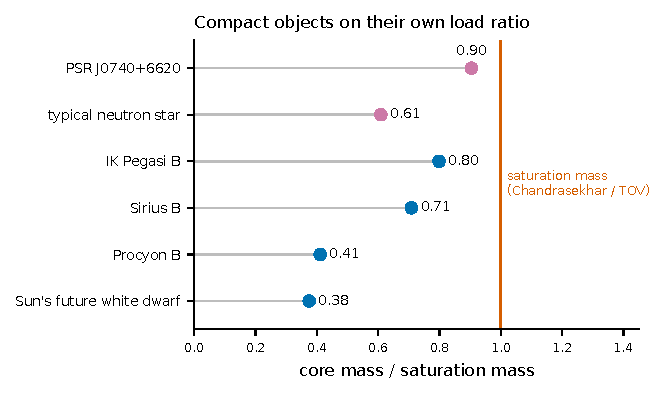
\includegraphics[width=0.8\textwidth]{figures/part4/fig_compact_objects.pdf}
\caption{Compact objects on their own load ratio, core mass over saturation mass (1.44~$M_\odot$ for white dwarfs; about
2.3~$M_\odot$ for neutron stars, which is uncertain). Masses as quoted in the author's notes. \calc{} for the ratios; the comparison
with cells is \analogy.}
\label{fig:compact}
\end{figure}
